\section{Introduction}
The main {\tt GitHub} link for this work is \url{https://github.com/aravindhv10/MUMBAIPUNETAUTAGGER}.
The latest version of this document can always be found at ``\url{https://github.com/aravindhv10/MUMBAIPUNETAUTAGGER/blob/master/HERWIG_PART/ReadME.pdf}''.
The sources for this document (including the figures in case you want to use them anywhere) can be found at ``\url{https://github.com/aravindhv10/MUMBAIPUNETAUTAGGER/tree/master/HERWIG_PART/Documentation}''.

\subsection{Installing Herwig-7}
To install Herwig, please make sure you have a {\bf proper} root installation (and source "{\tt thisroot.sh}" if it is installed in non-standard location) as Herwig uses {\tt libpyroot}.
Download and install {\tt Herwig} by running the script \url{https://herwig.hepforge.org/herwig-bootstrap}:
\begin{center}
    \begin{minipage}{0.7\textwidth}
        {\tt
            wget -c '\url{https://herwig.hepforge.org/herwig-bootstrap}'\\
            chmod +x './herwig-bootstrap'\\
            './herwig-bootstrap' './HerwigInstall'
        }
    \end{minipage}
\end{center}
This will install {\tt Herwig} to the location `{\tt ./HerwigInstall}' along with all of it's dependencies ({\tt boost}, {\tt fastjet}, {\tt HepMC}, etc).
Full instructions for using this script is found in \url{https://herwig.hepforge.org/tutorials/installation/bootstrap.html}.

\section{Generating events:}
\subsection{The Partonic Level Events:}
The quickest way I could find to generate events in {\tt Herwig} was by generating parton level events in {\tt MadGraph} and shower using {\tt Herwig} (I also got suggestions to adopt similar method for {\tt Pythia} as this nicely isolates matrix element generation from showering and our main aim is the study effect of different showering and hadronization techniques on our jet substructure algorithms).
\begin{center}
    \begin{minipage}{0.7\textwidth}
        { \tt
            wget -c '\url{https://launchpad.net/mg5amcnlo/2.0/2.6.x/+download/MG5_aMC_v2.6.1.tar.gz}';\\
            tar -xf "MG5\_aMC\_v2.6.1.tar.gz";\\
            cd "MG5\_aMC\_v2\_6\_1/";\\
            ./bin/mg5\_aMC
        }
    \end{minipage}
\end{center}
This will start madgraph, now you can generate LHE files:
\begin{center}
    \begin{minipage}{0.7\textwidth}
        {\tt
            generate p p > z j\\
            output zj\\
            exit
        }
    \end{minipage}
\end{center}
Once you are done with above steps, {\tt MadGraph} exits, now you will need to edit some configuration files:
\begin{center}
    \begin{minipage}{0.7\textwidth}
        {\tt
            cd zj/Cards/\\
            <editor> 'run\_card.dat'\\
        }
    \end{minipage}
\end{center}
Where, {\tt <editor>} stands for any text editor. You will need to change the following in the file:
\begin{center}
    \begin{minipage}{0.7\textwidth}
        {\tt 0.0  = ptheavy   ! minimum pt for at least one heavy final state}
    \end{minipage}
\end{center}
To the value desired, we will pick this to be 200 GeV.
\begin{center}
    \begin{minipage}{0.7\textwidth}
        {\tt 200.0  = ptheavy   ! minimum pt for at least one heavy final state}
    \end{minipage}
\end{center}
Next edit {\tt madspin\_card\_default.dat} and change the line:
\begin{center}
    \begin{minipage}{0.7\textwidth}
        {\tt decay z > all all}
    \end{minipage}
\end{center}
to:
\begin{center}
    \begin{minipage}{0.7\textwidth}
        {\tt decay z > ta- ta+}
    \end{minipage}
\end{center}
now madgraph is set up and can be run, in the shell:
\begin{center}
    \begin{minipage}{0.7\textwidth}
        {\tt
            cd ../;\\
            ./bin/generate\_events
        }
    \end{minipage}
\end{center}
Once you get the {\tt MadGraph} prompt:
\begin{center}
    \begin{minipage}{0.7\textwidth}
        {\tt
            4\\
            0\\
            0
        }
    \end{minipage}
\end{center}
Now note the “4” is important, you will need to run with {\tt MadSpin}
(to force $Z {\rightarrow} {\tau} \bar{\tau}$ decays) once you are done, you will have the LHE files in:
\begin{center}
    \begin{minipage}{0.7\textwidth}
        {\tt ./Events/run\_01\_decayed\_1/unweighted\_events.lhe.gz}
    \end{minipage}
\end{center}
you can extract this:
\begin{center}
    \begin{minipage}{0.7\textwidth}
        {\tt gzip -d "./Events/run\_01\_decayed\_1/unweighted\_events.lhe.gz"}
    \end{minipage}
\end{center}

The complete list of LHE files generated using the above methods can be downloaded from ``\url{https://drive.google.com/file/d/1sVQSYUDPqSB0vgh84Y8IIOucBSMMr9rL/view?usp=sharing}''

\subsection{Showering:}
Move the LHE file to another directory where you want to do the showering:
\begin{center}
    \begin{minipage}{0.8\textwidth}
        {\tt
            mkdir  \textasciitilde/shower;\\
            cp "./Events/run\_01\_decayed\_1/unweighted\_events.lhe" \textasciitilde/shower/1.lhe
        }
    \end{minipage}
\end{center}
now you will need to activate {\tt Herwig} (note, {\tt <HerwigInstall>} needs to be replaced by the correct directory):
\begin{center}
    \begin{minipage}{0.7\textwidth}
        {\tt source <HerwigInstall>/bin/activate}
    \end{minipage}
\end{center}

Once this is done, download the file ``\url{https://github.com/aravindhv10/MUMBAIPUNETAUTAGGER/blob/master/HERWIG_PART/LHEWithISR.in}'' to the current directory (\textasciitilde/shower). In LHE.in, edit the line:
\begin{center}
    \begin{minipage}{0.7\textwidth}
        {\tt set LesHouchesReader:FileName unweighted\_events.lhe}
    \end{minipage}
\end{center}
and change ``{\tt unweighted\_events.lhe}'' to the LHE file you want to shower.
You can also edit the PDF choices if you want (note that you may need to download the appropriate pdf fits manually using {\tt lhapdf} installed in the {\tt <HerwigInstall>} directory).

note that the lines
\begin{center}
    \begin{minipage}{0.7\textwidth}
        {\tt
            read snippets/HepMC.in\\
            set /Herwig/Analysis/HepMC:PrintEvent 100
        }
    \end{minipage}
\end{center}
is responsible for producing the {\tt HepMC} file, you can then use {\tt Delphes} on these files. We are done. Now run {\tt Herwig}:
\begin{center}
    \begin{minipage}{0.7\textwidth}
        {\tt
            Herwig read LHE.in\\
            Herwig run LHE.in
        }
    \end{minipage}
\end{center}
You can change underlying event, tunes, etc in the LHE.in file, explore \url{https://herwig.hepforge.org/tutorials/faq/shower.html} for details.

By default, {\tt Herwig} does not force $\tau$ to decay hadronically. This can be forced, check the link: \url{https://herwig.hepforge.org/tutorials/faq/decay.html} to know how this can be done. Basically you would need:
\begin{center}
    \begin{minipage}{0.8\textwidth}
        {\tt
            set /Herwig/Particles/tau+/tau+->nu\_taubar,nu\_e,e+;:OnOff Off\\
            set /Herwig/Particles/tau+/tau+->nu\_taubar,nu\_mu,mu+;:OnOff Off\\
            set /Herwig/Particles/tau-/tau-->nu\_tau,nu\_ebar,e-;:OnOff Off\\
            set /Herwig/Particles/tau-/tau-->nu\_tau,nu\_mubar,mu-;:OnOff Off
        }
    \end{minipage}
\end{center}

A sample card to run with (\url{https://github.com/aravindhv10/MUMBAIPUNETAUTAGGER/blob/master/HERWIG_PART/LHEWithISR.in}) and without (\url{https://github.com/aravindhv10/MUMBAIPUNETAUTAGGER/blob/master/HERWIG_PART/LHENoISRMPI.in}) mpi is available in the {\tt GitHub} page.

Example for an extremely simple reader is available in \url{https://github.com/aravindhv10/MUMBAIPUNETAUTAGGER/tree/master/COMMON/DelphesReader}.

\section{Reading the root files and some results:}

We use the following color convention for graphs through out the document:
\begin{center}
    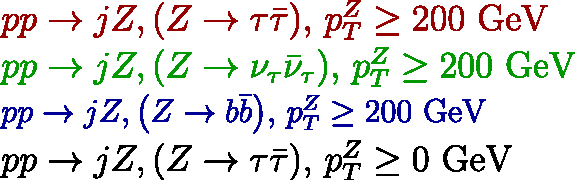
\includegraphics[width=0.5\textwidth]{./ColorConventions.pdf}
\end{center}
The main reader program can be found at ``\url{https://github.com/aravindhv10/MUMBAIPUNETAUTAGGER/tree/master/COMMON/DelphesReader}''.
We present some simple results obtained using these methods (Note: we use the BDRS+filtering method on the jet to identify hard substructures and consider events with MPI enabled).

\begin{figure}
    \begin{center}
        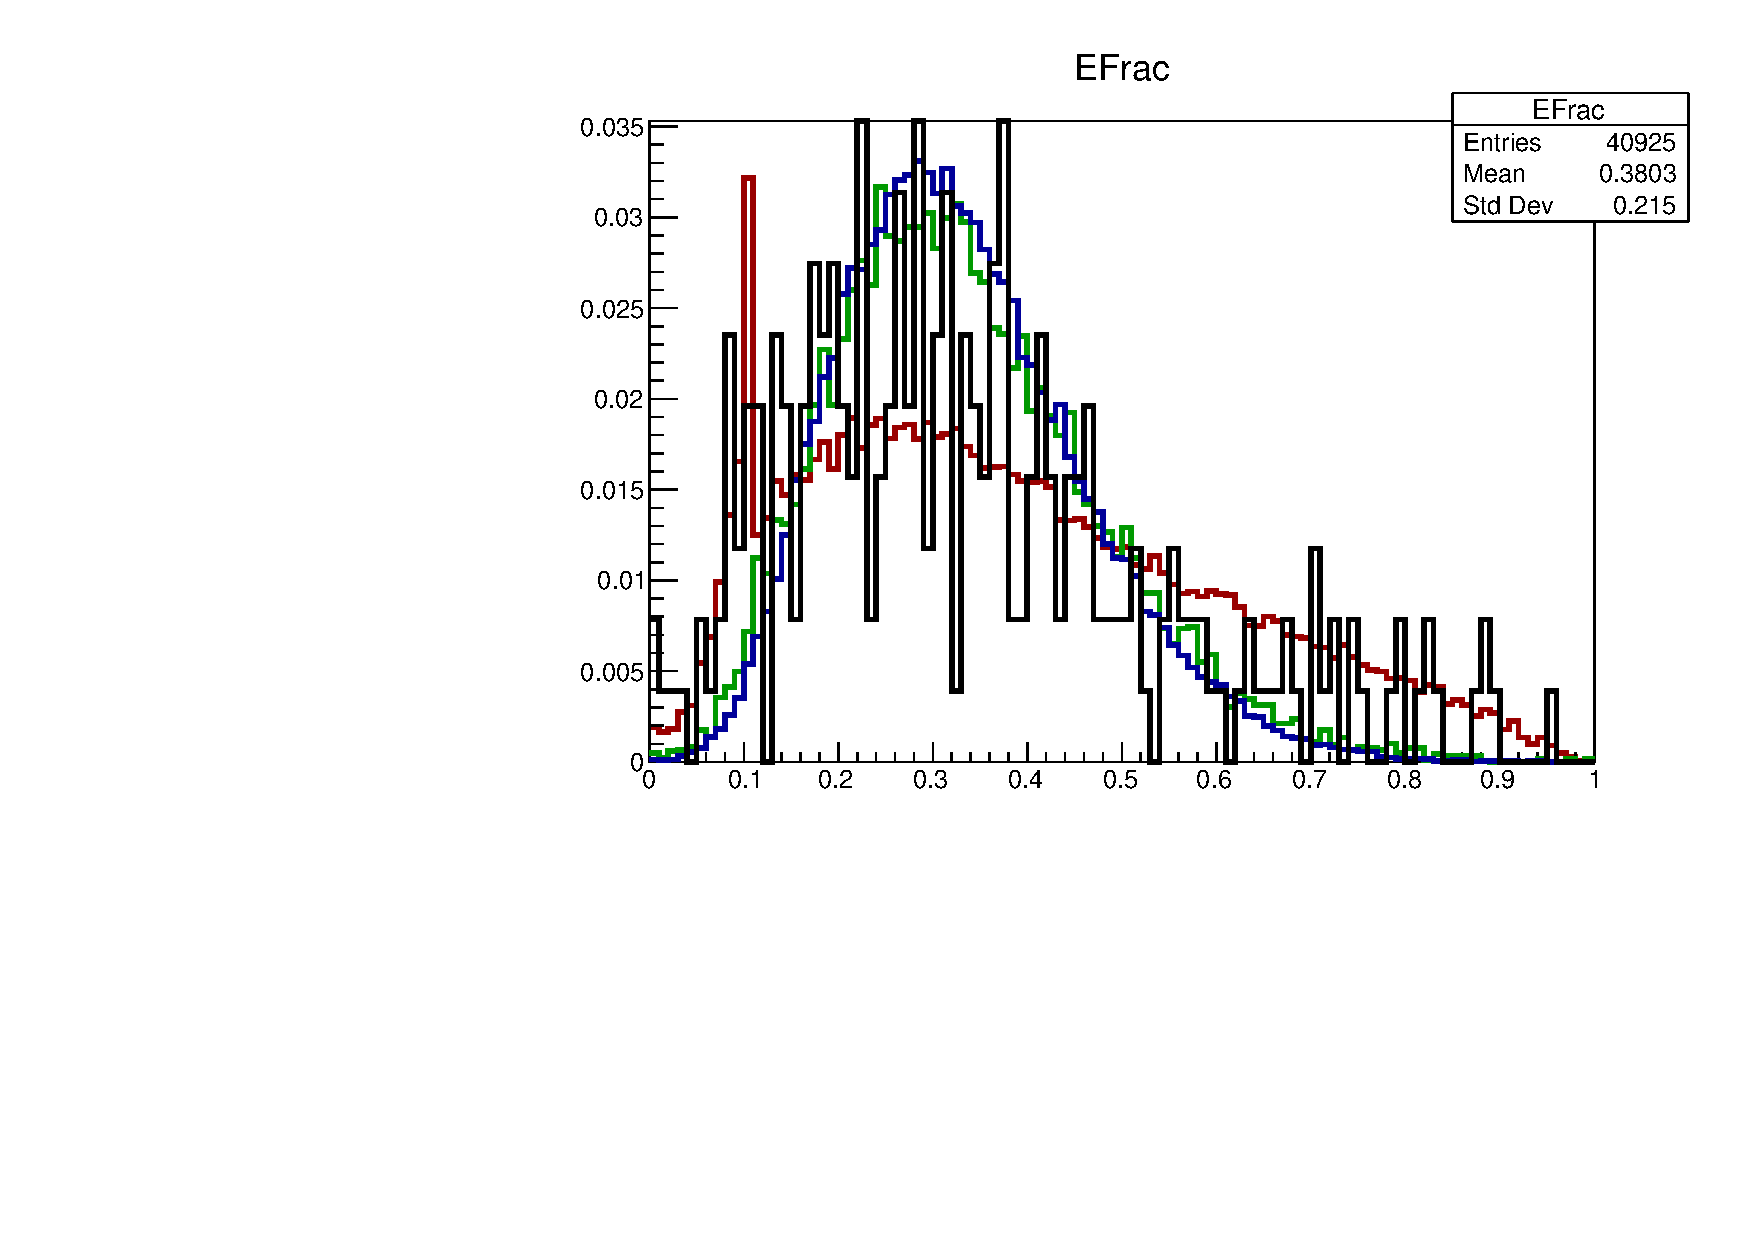
\includegraphics[width=0.7\textwidth]{./EFrac.pdf}
        \caption{ Electromagnetic energy fraction of the jet, normalized to unit area under the curve. }
        \label{fig:EFrac}
    \end{center}
\end{figure}

\begin{figure}
    \begin{center}
        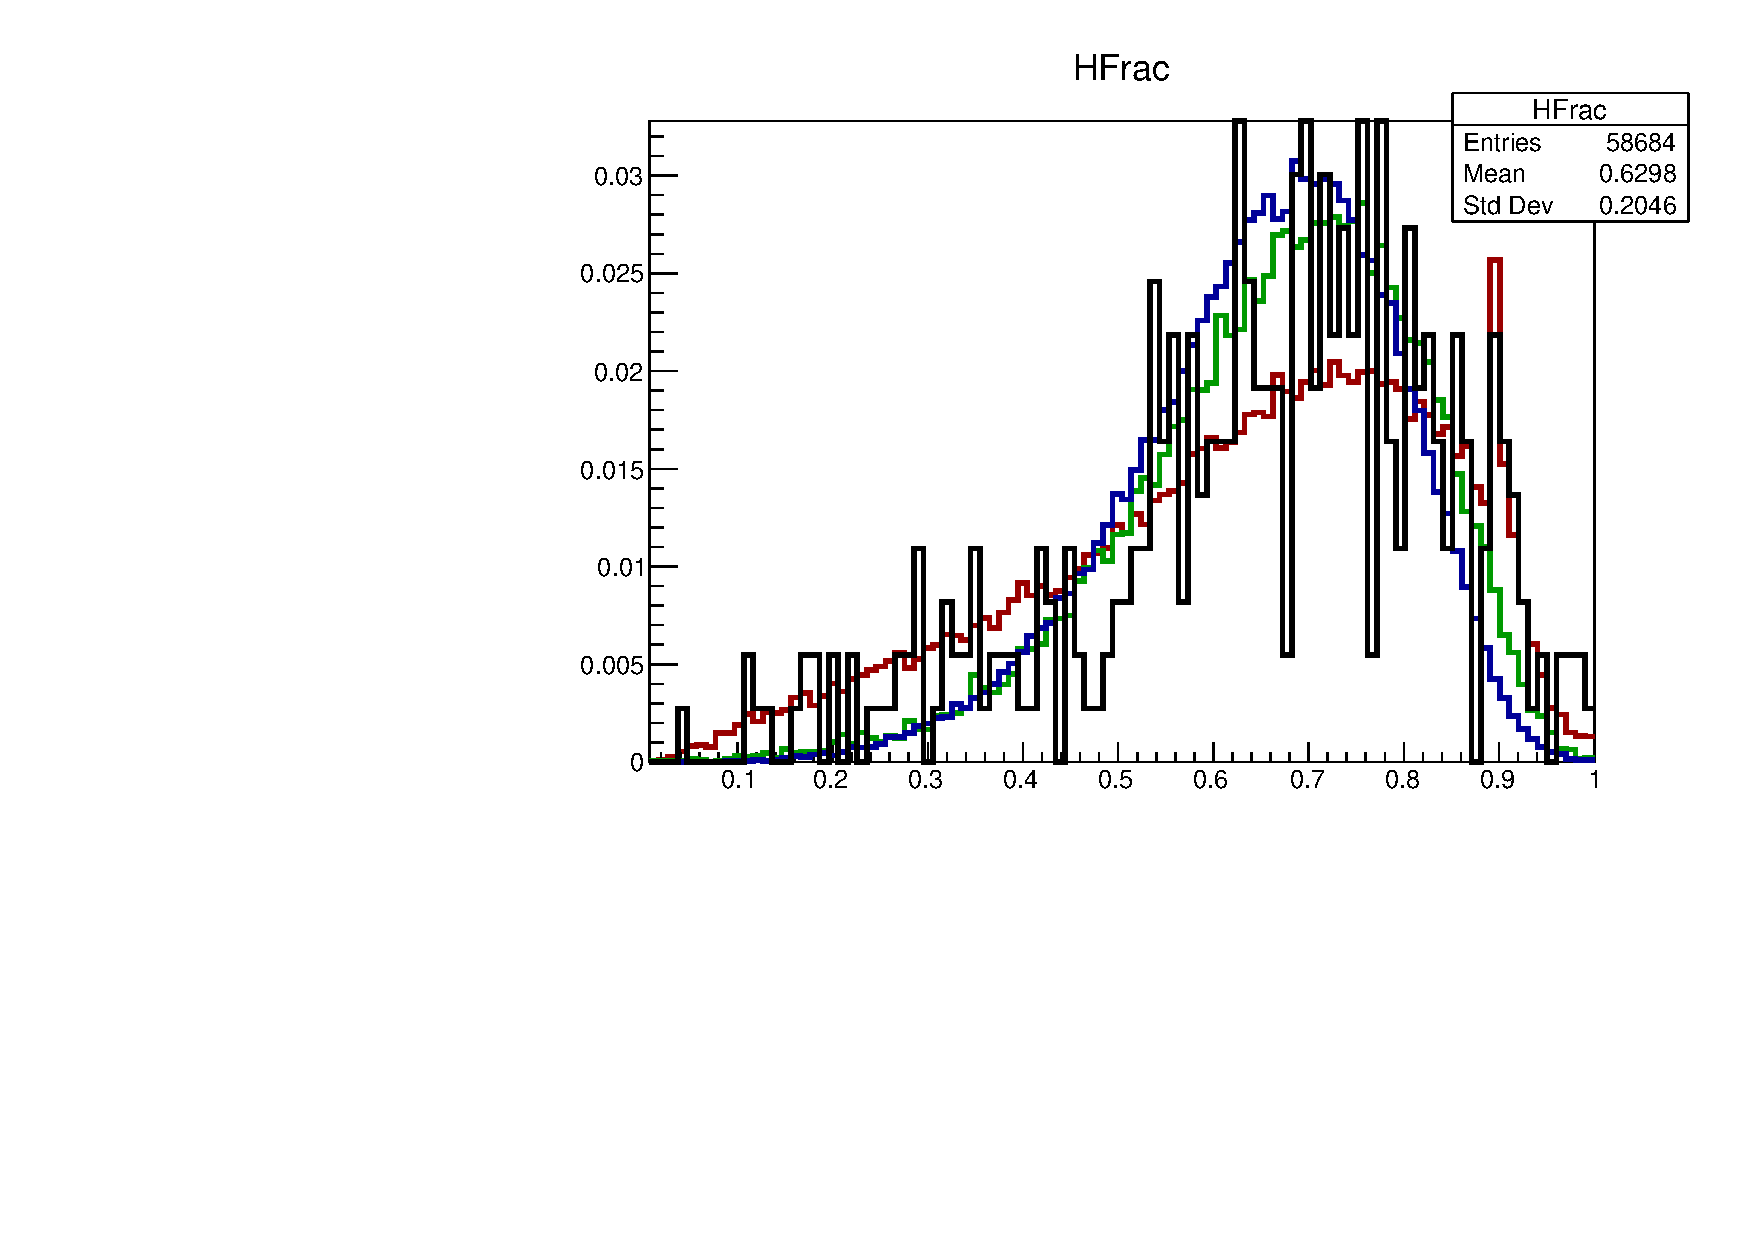
\includegraphics[width=0.7\textwidth]{./HFrac.pdf}
        \caption{ Hadronic energy fraction of the jet, normalized to unit area under the curve. }
        \label{fig:HFrac}
    \end{center}
\end{figure}

\begin{figure}
    \begin{center}
        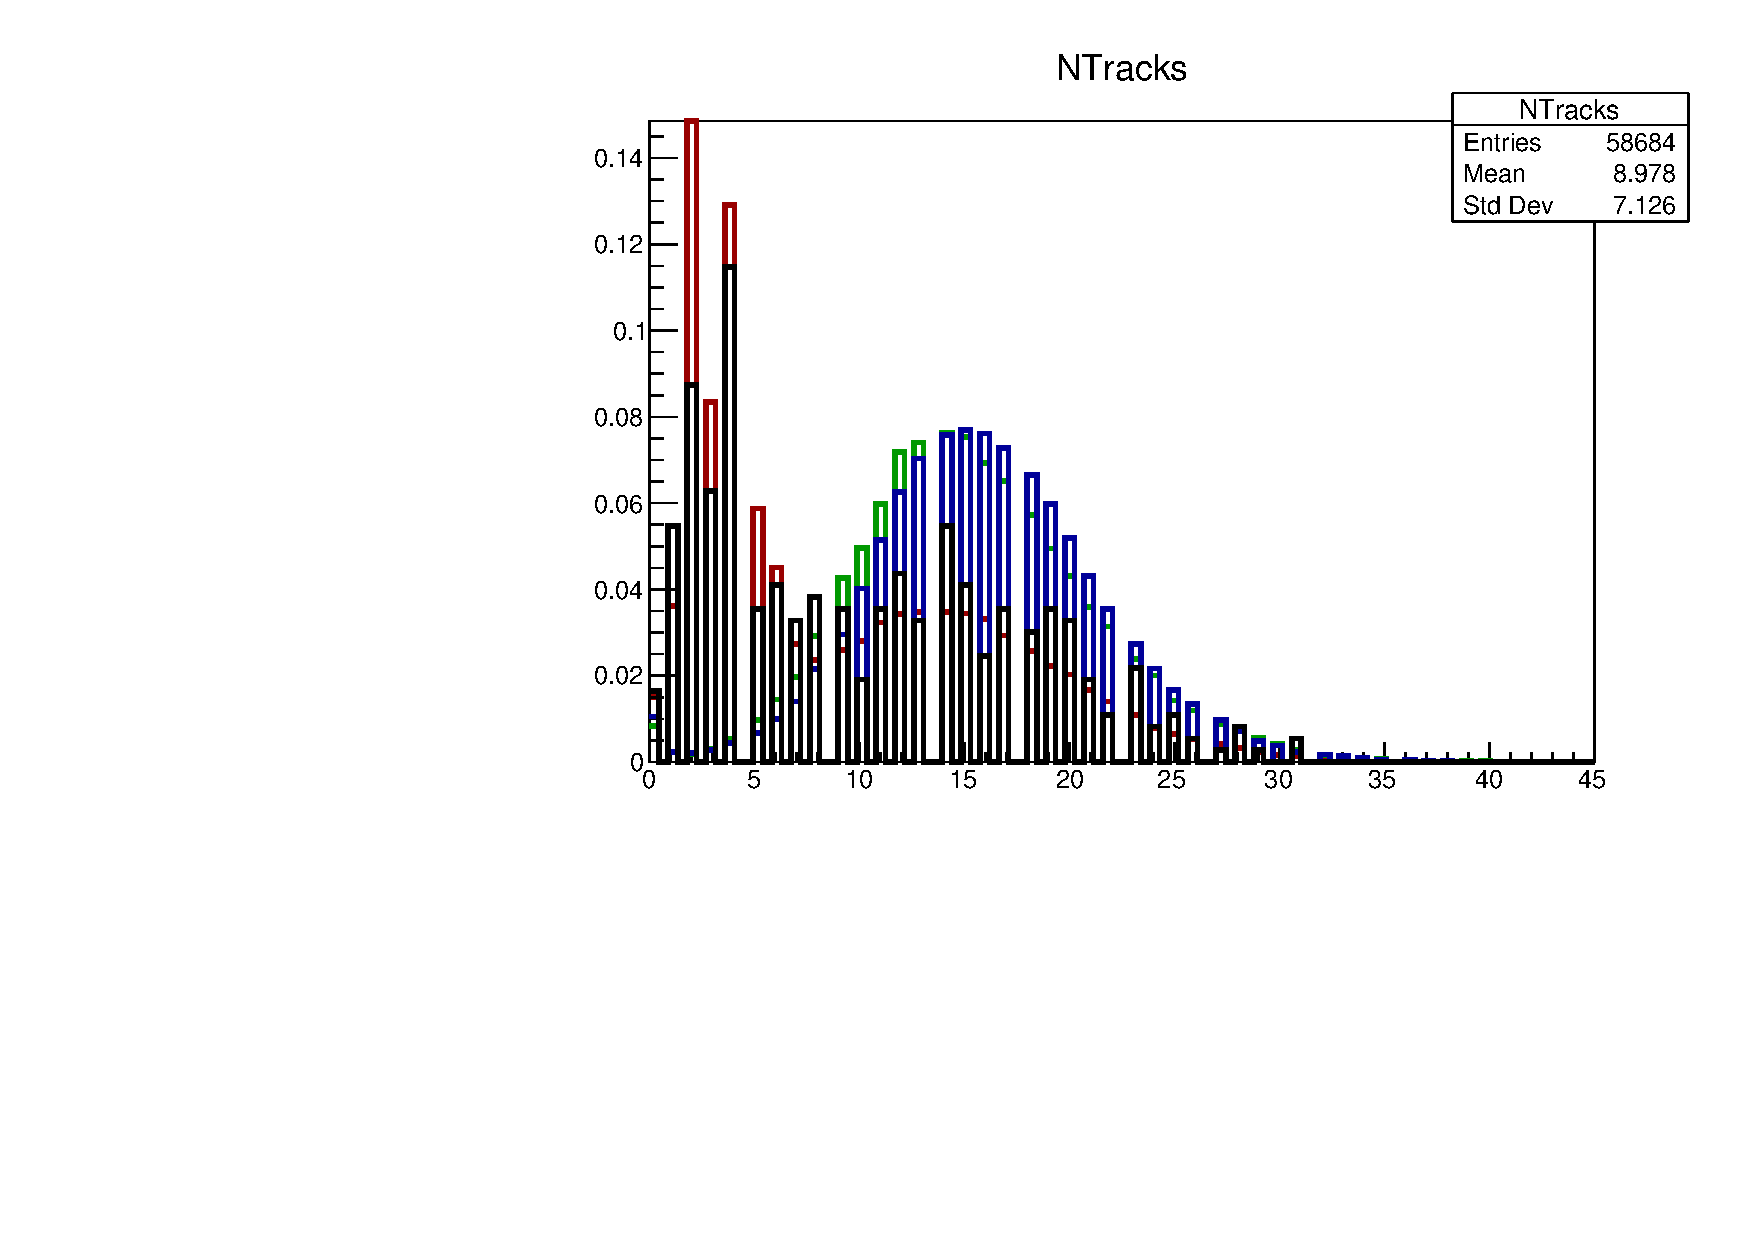
\includegraphics[width=0.7\textwidth]{./NTracks.pdf}
        \caption{ Number of tracks in the jet, normalized to unit area under the curve. }
        \label{fig:NTracks}
    \end{center}
\end{figure}

\begin{figure}
    \begin{center}
        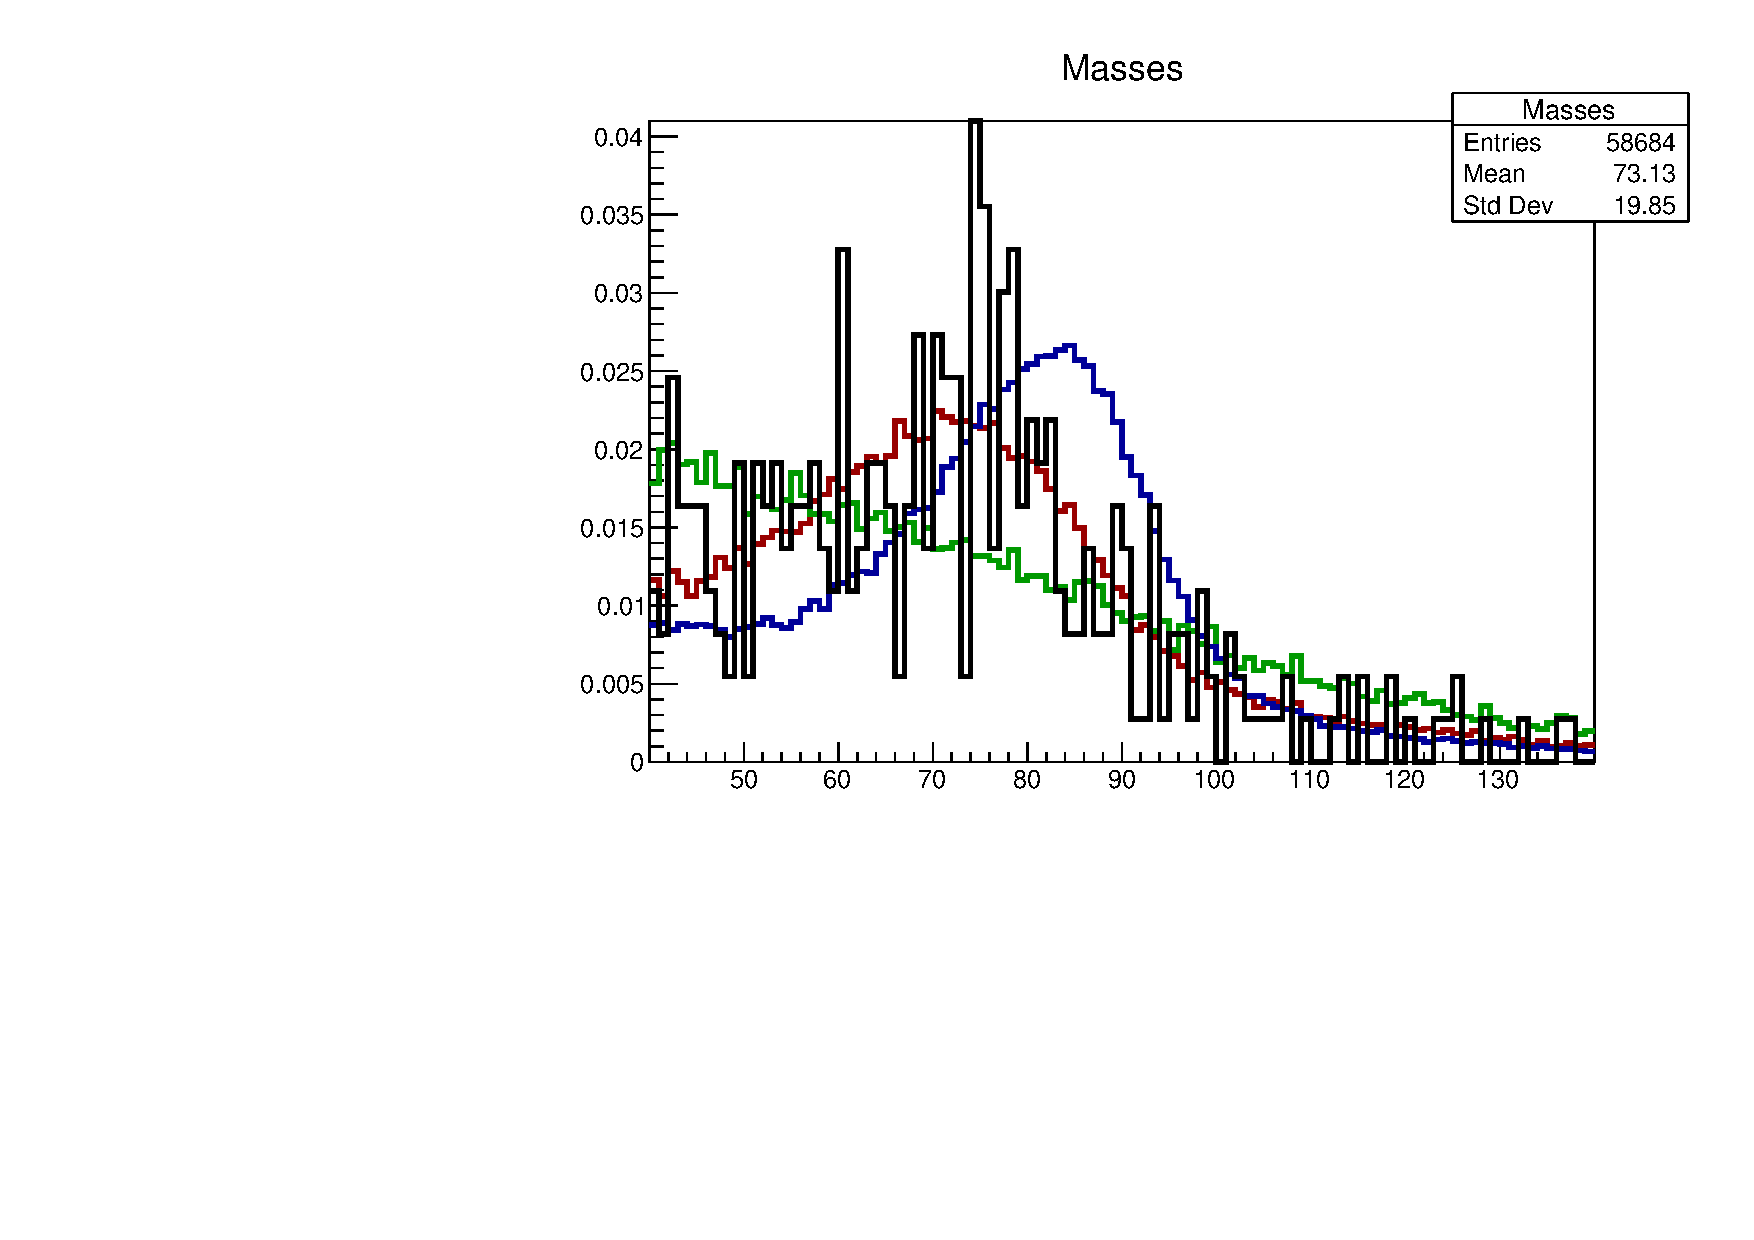
\includegraphics[width=0.7\textwidth]{./Masses.pdf}
        \caption{ Masses of the jet after BDRS and filtering steps, normalized to unit area under the curve. }
        \label{fig:Masses}
    \end{center}
\end{figure}

\begin{figure}
    \begin{center}
        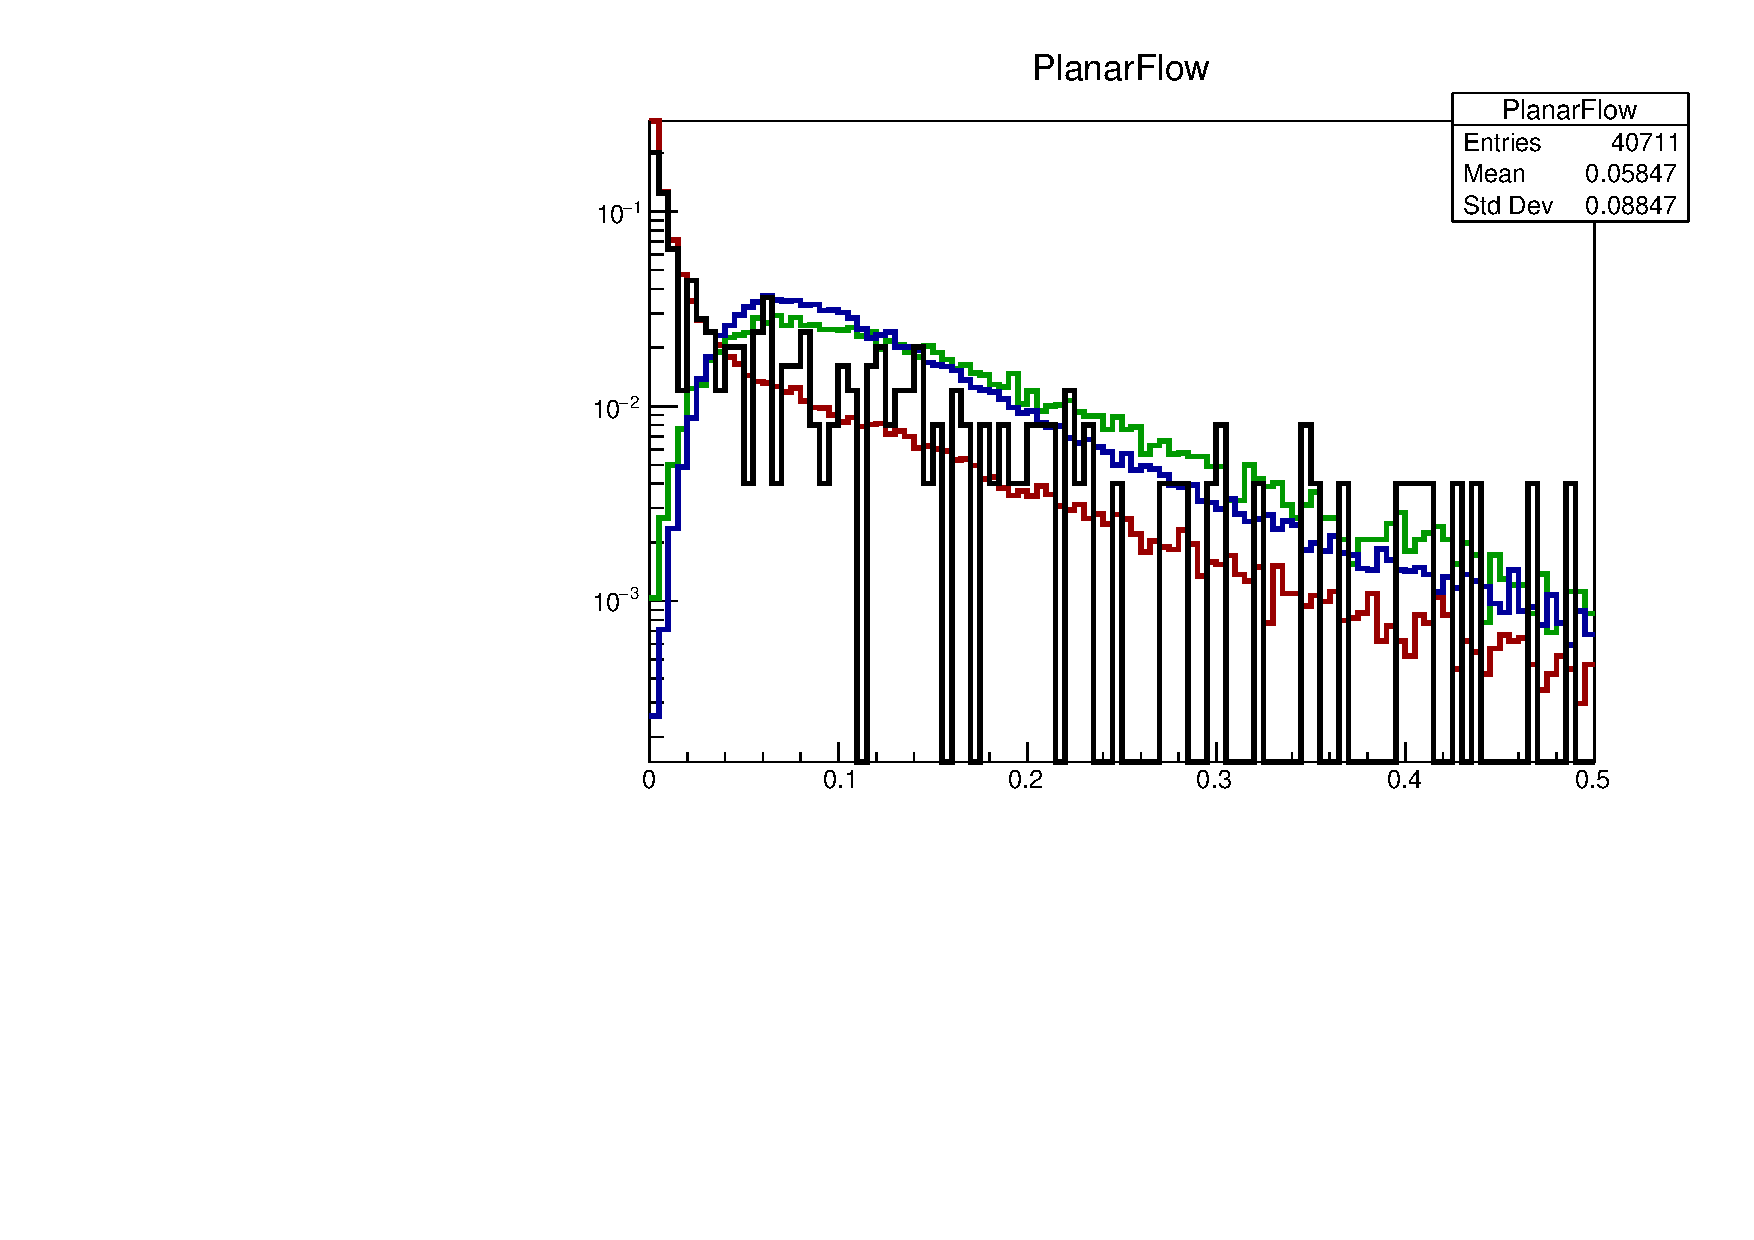
\includegraphics[width=0.7\textwidth]{./PlanarFlow.pdf}
        \caption{ Planar Flow of the jet after BDRS and filtering steps, normalized to unit area under the curve. }
        \label{fig:PlanarFlow}
    \end{center}
\end{figure}

\begin{figure}
    \begin{center}
        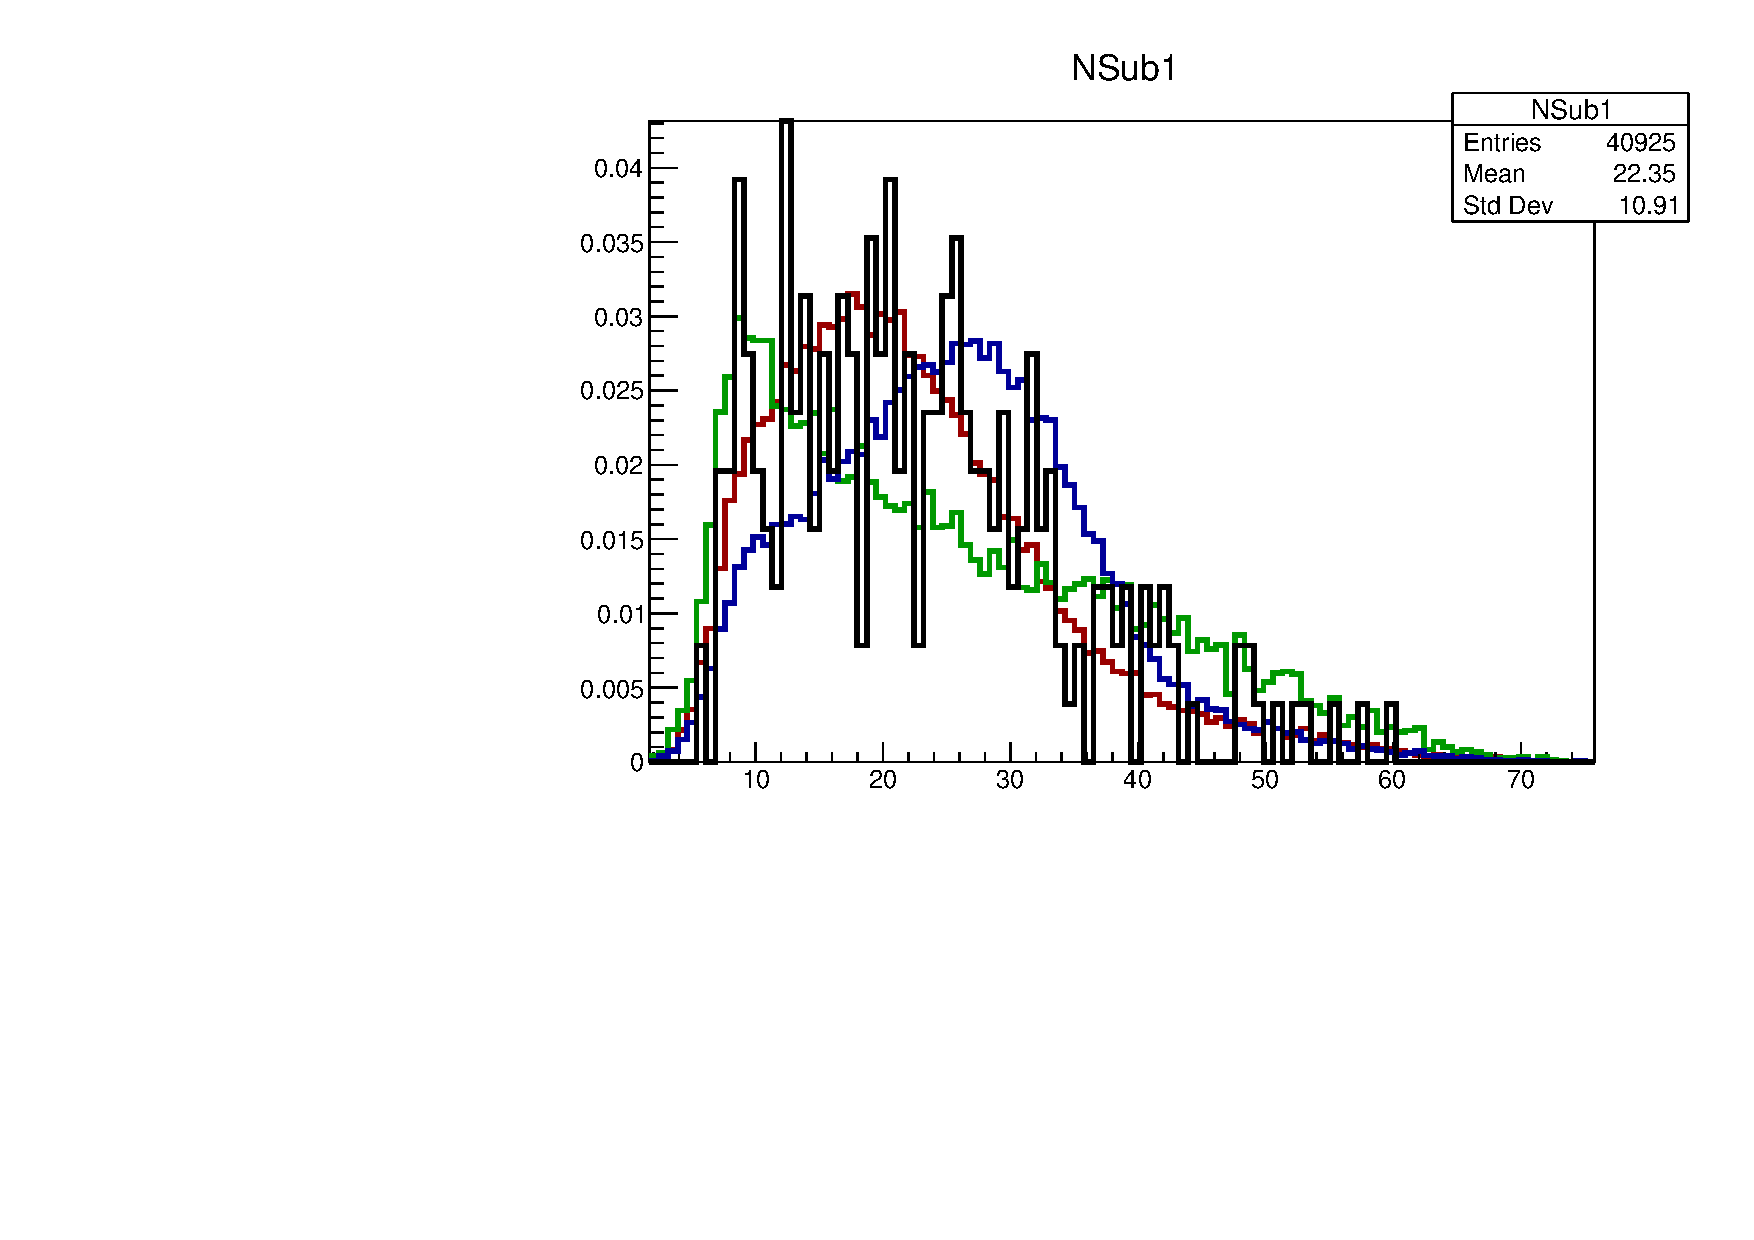
\includegraphics[width=0.49\textwidth]{./NSub1.pdf}
        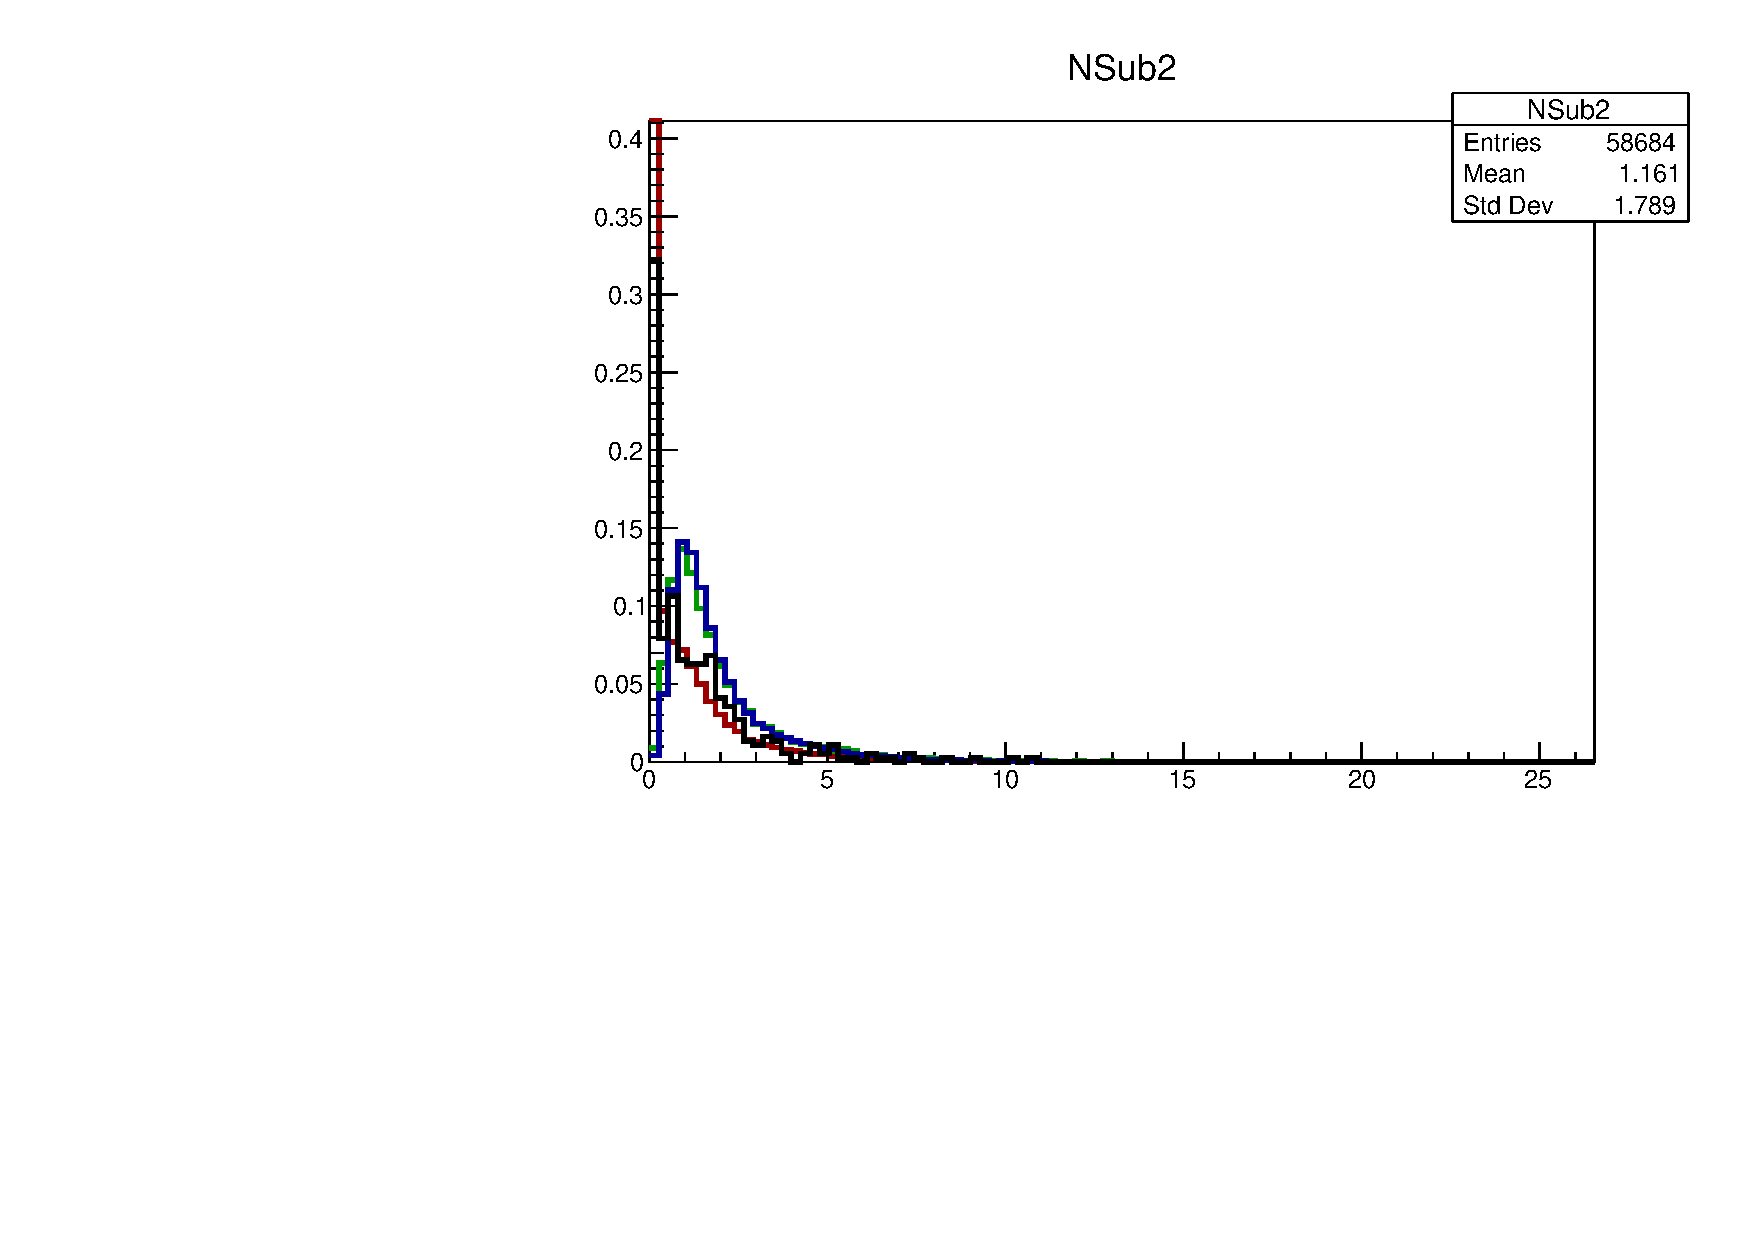
\includegraphics[width=0.49\textwidth]{./NSub2.pdf}\\
        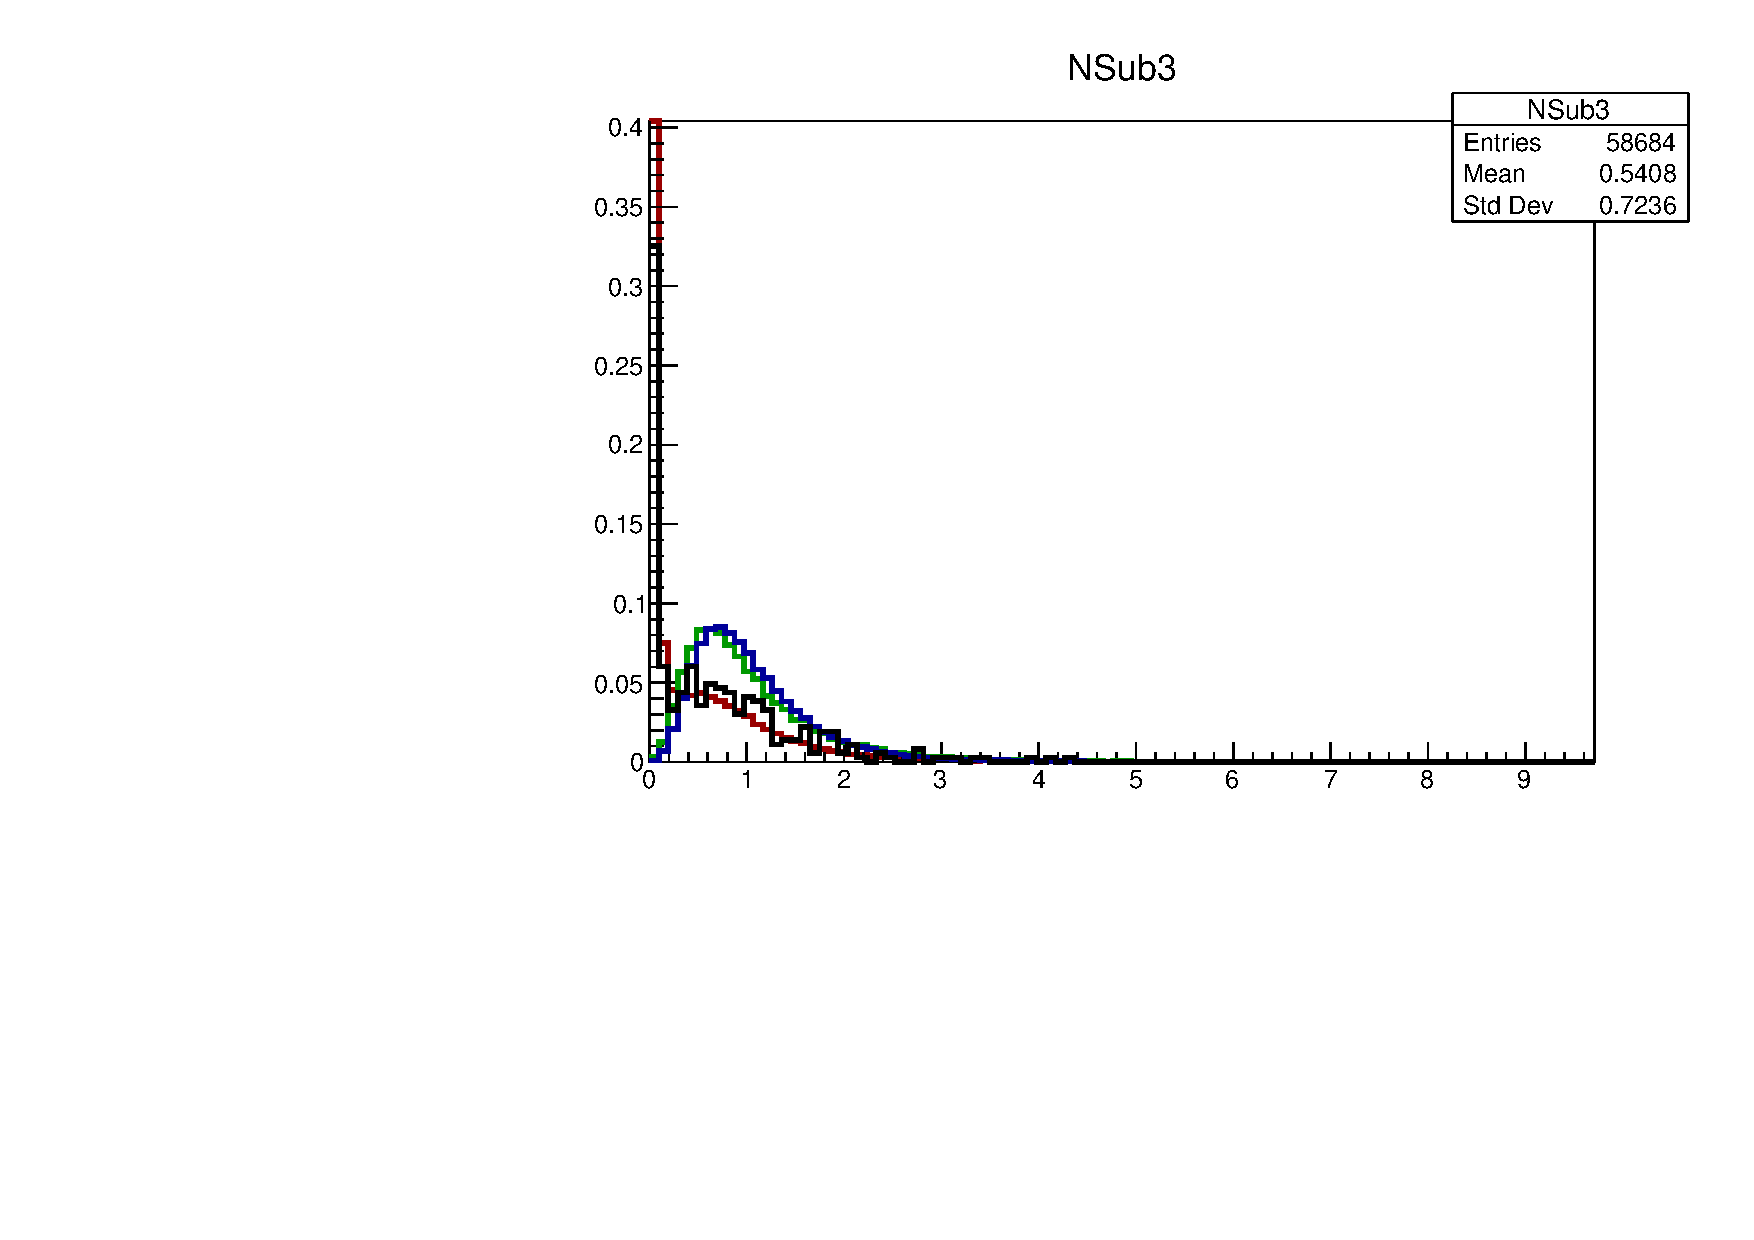
\includegraphics[width=0.49\textwidth]{./NSub3.pdf}
        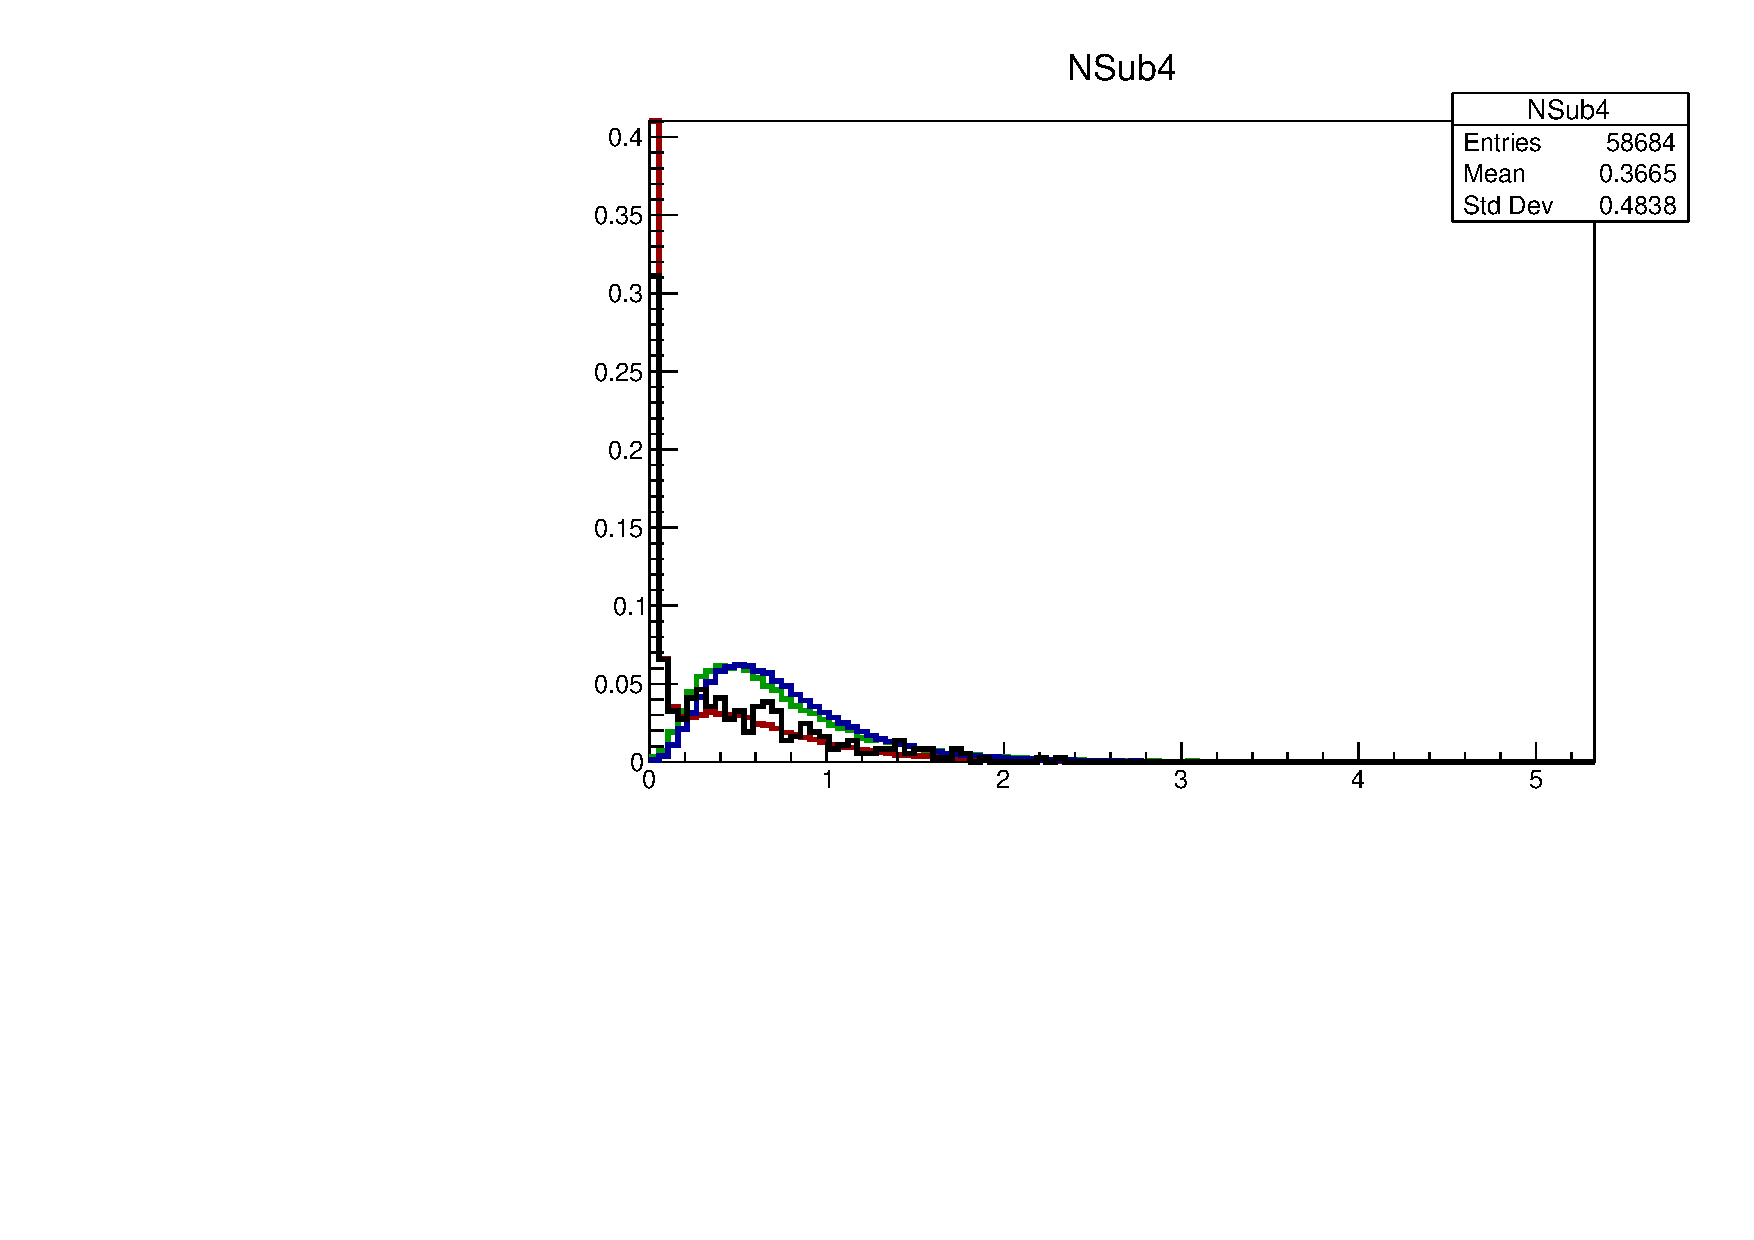
\includegraphics[width=0.49\textwidth]{./NSub4.pdf}\\
        \caption{ {\tt NSubJettiness} observable, normalized to unit area under the curve. }
        \label{fig:NSub}
    \end{center}
\end{figure}

\begin{figure}
    \begin{center}
        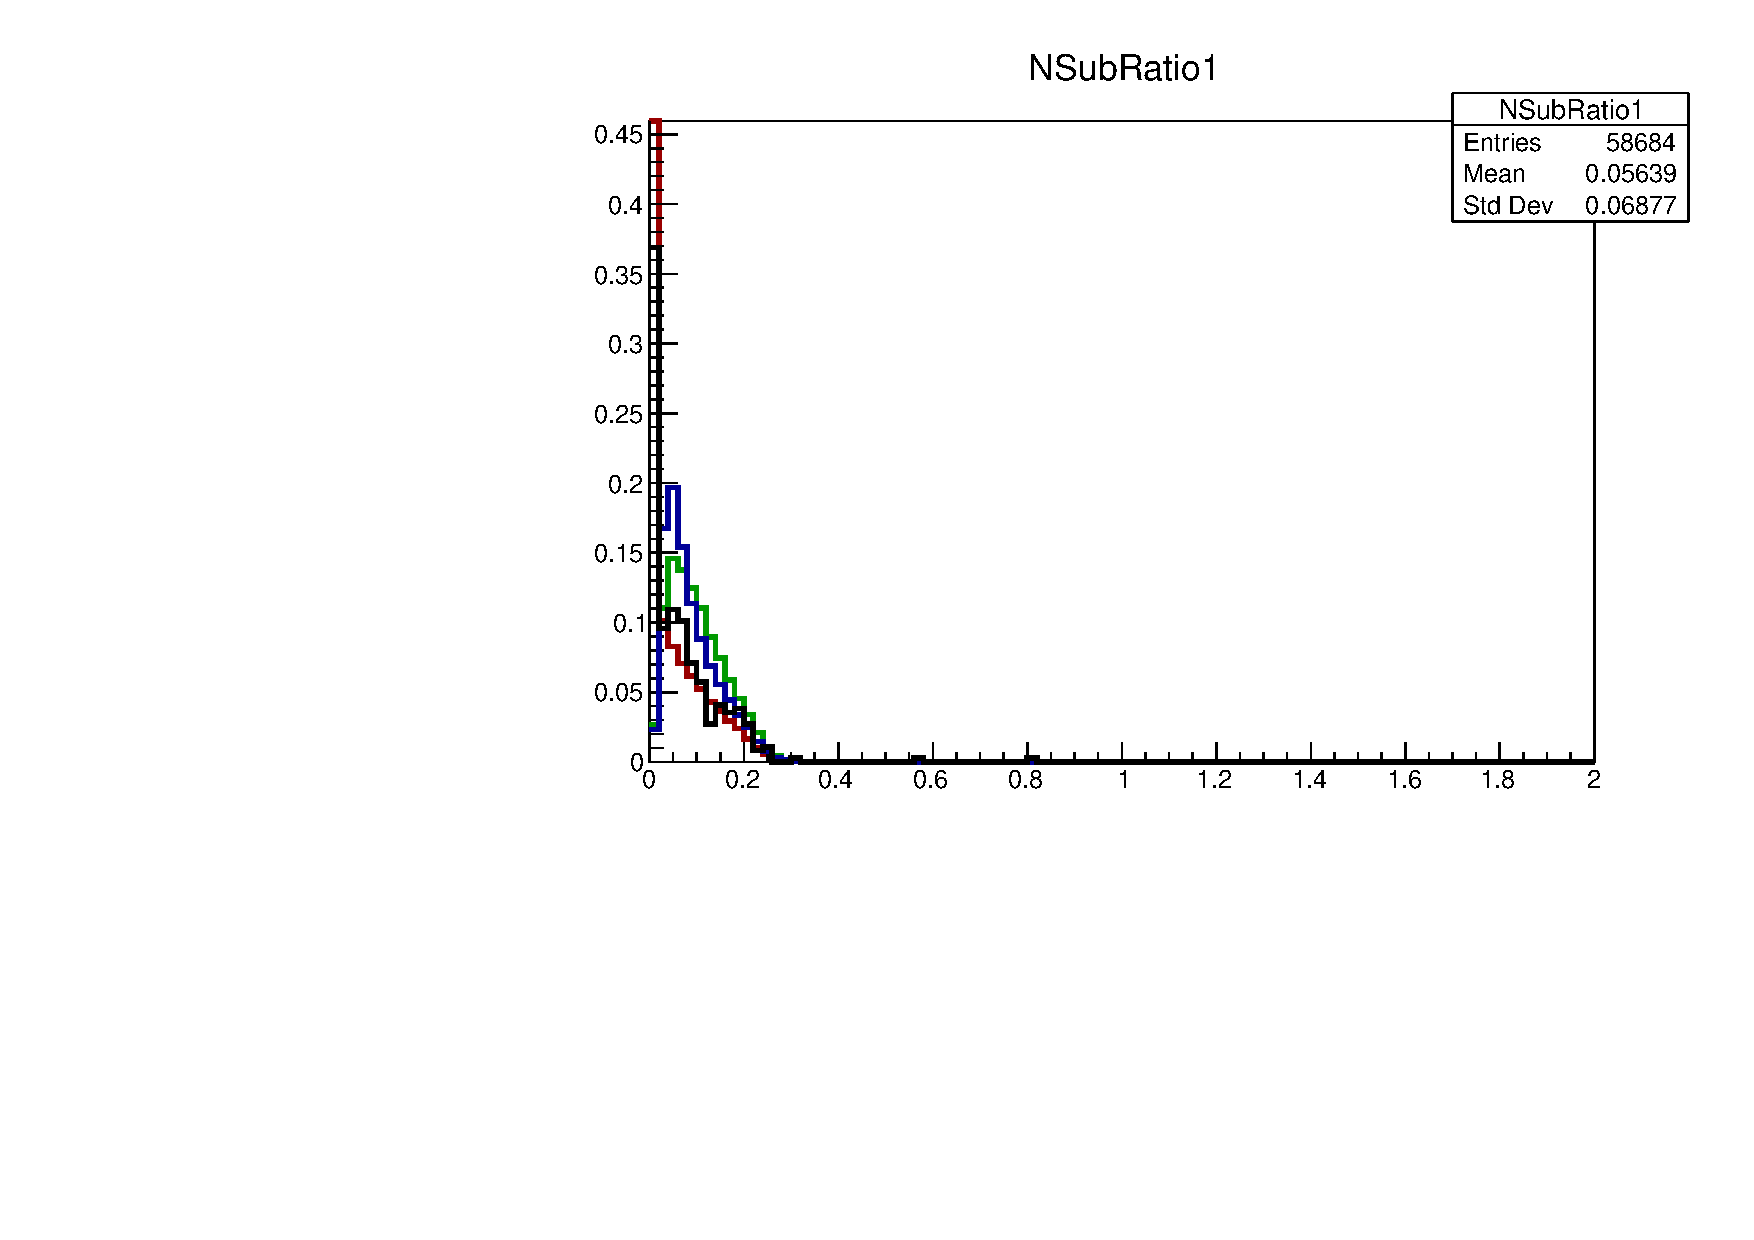
\includegraphics[width=0.49\textwidth]{./NSubRatio1.pdf}
        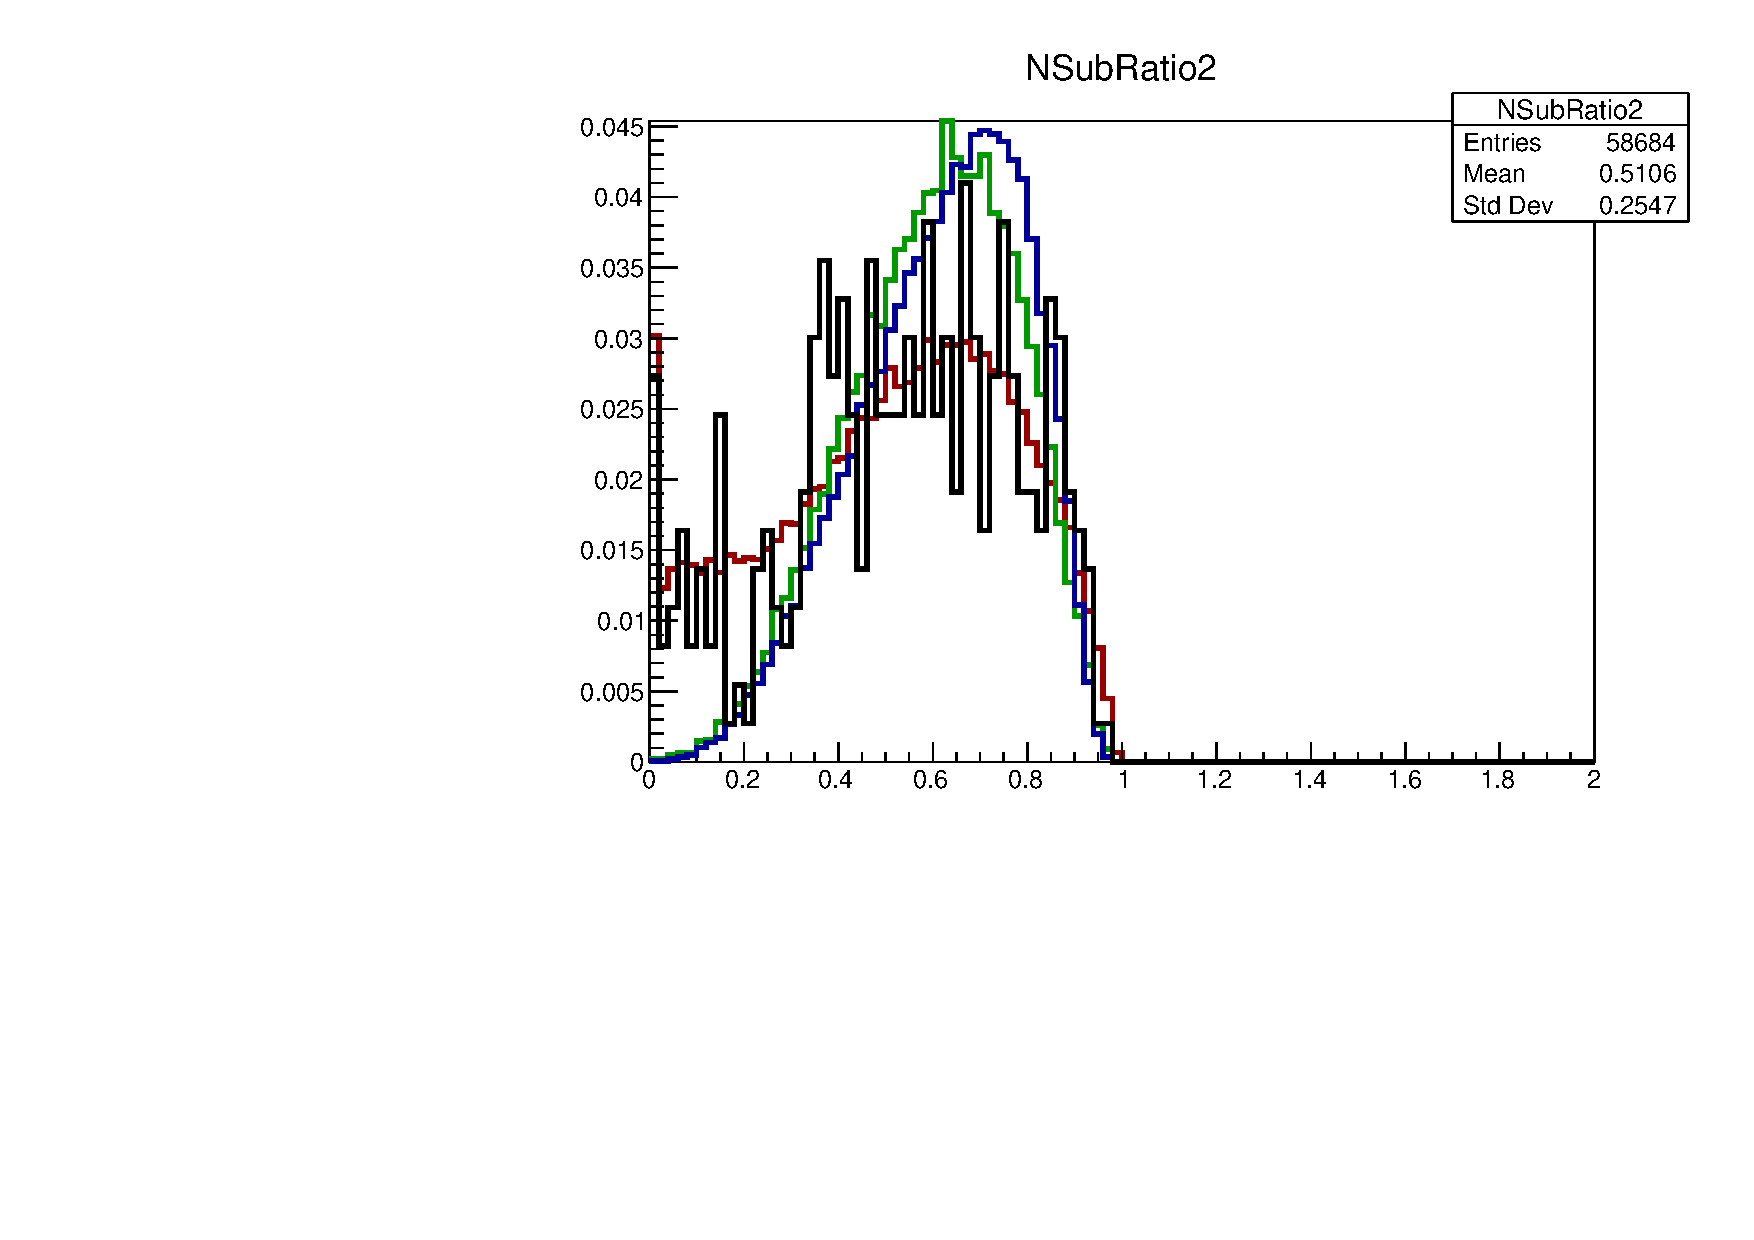
\includegraphics[width=0.49\textwidth]{./NSubRatio2.pdf}\\
        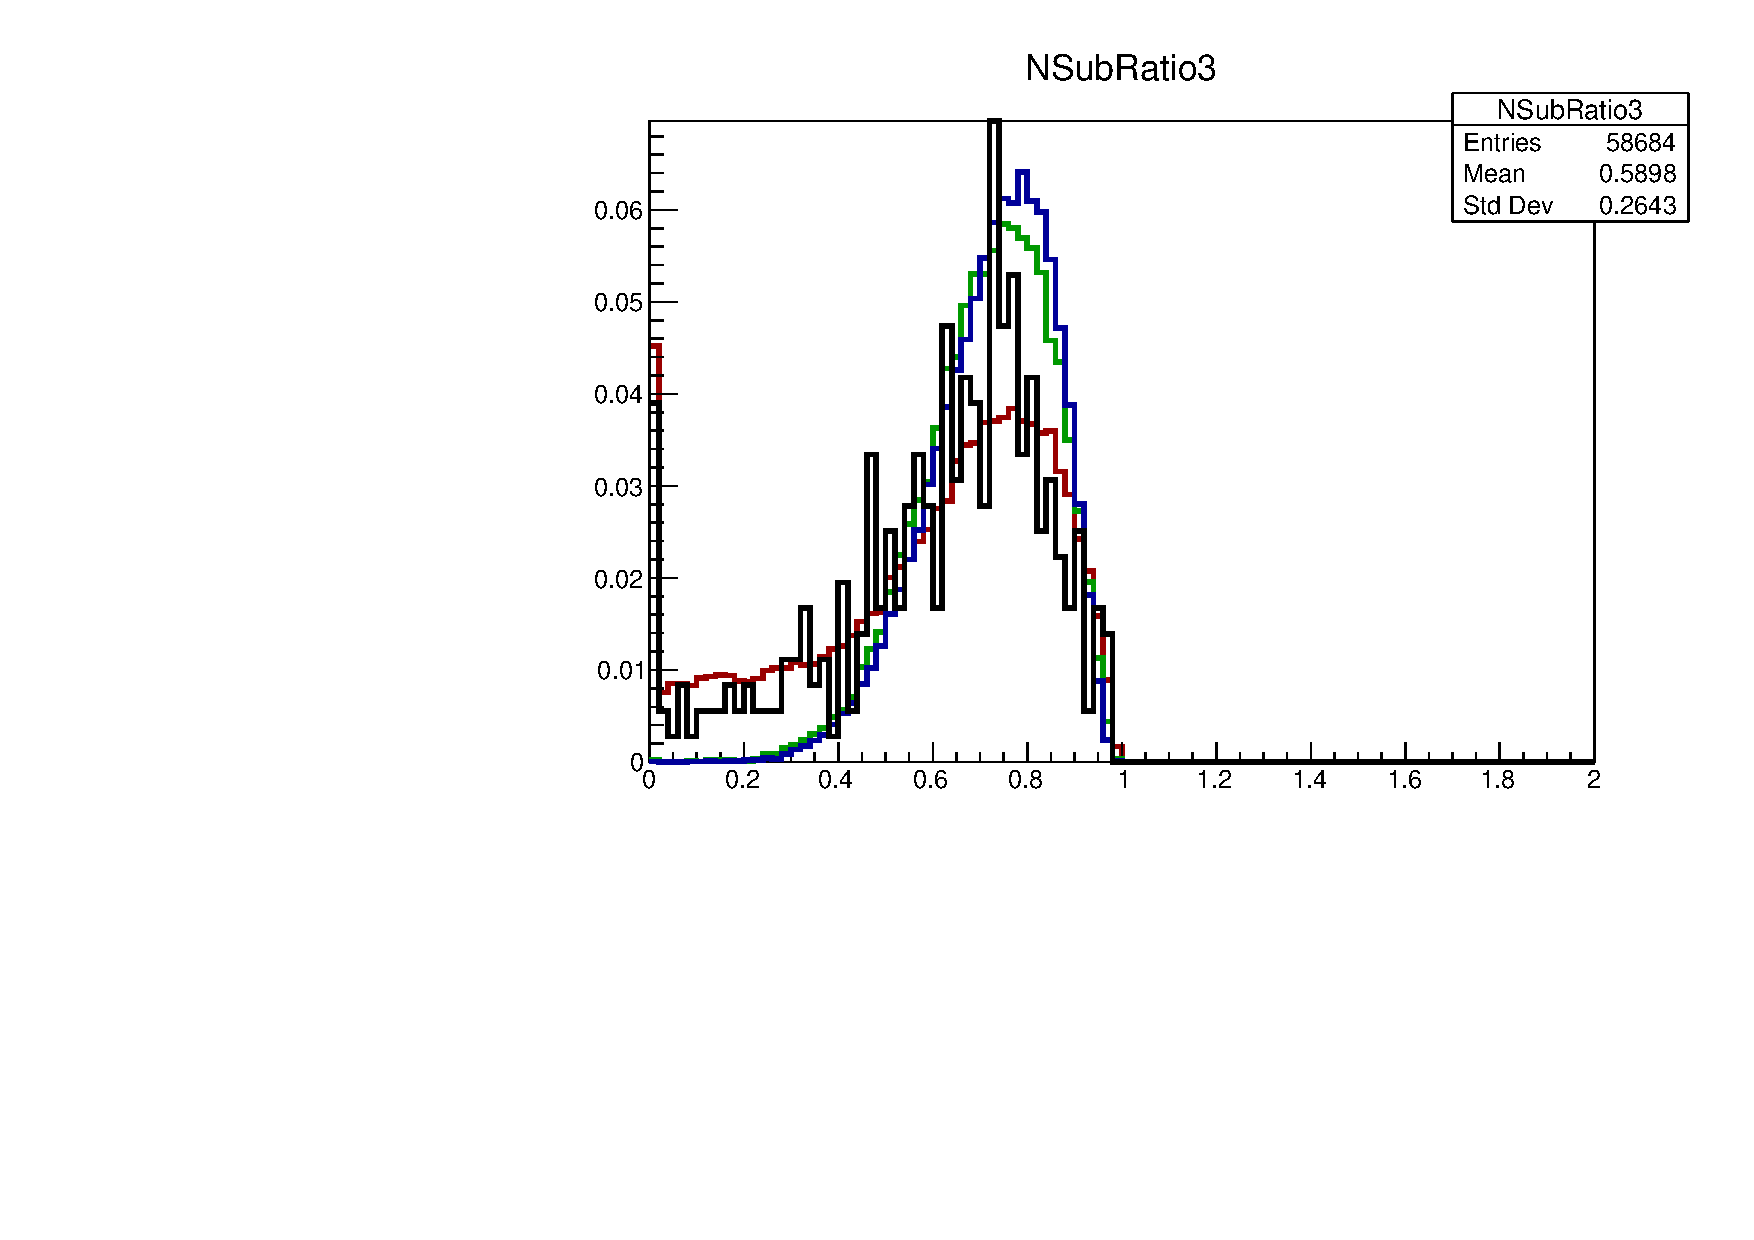
\includegraphics[width=0.49\textwidth]{./NSubRatio3.pdf}
        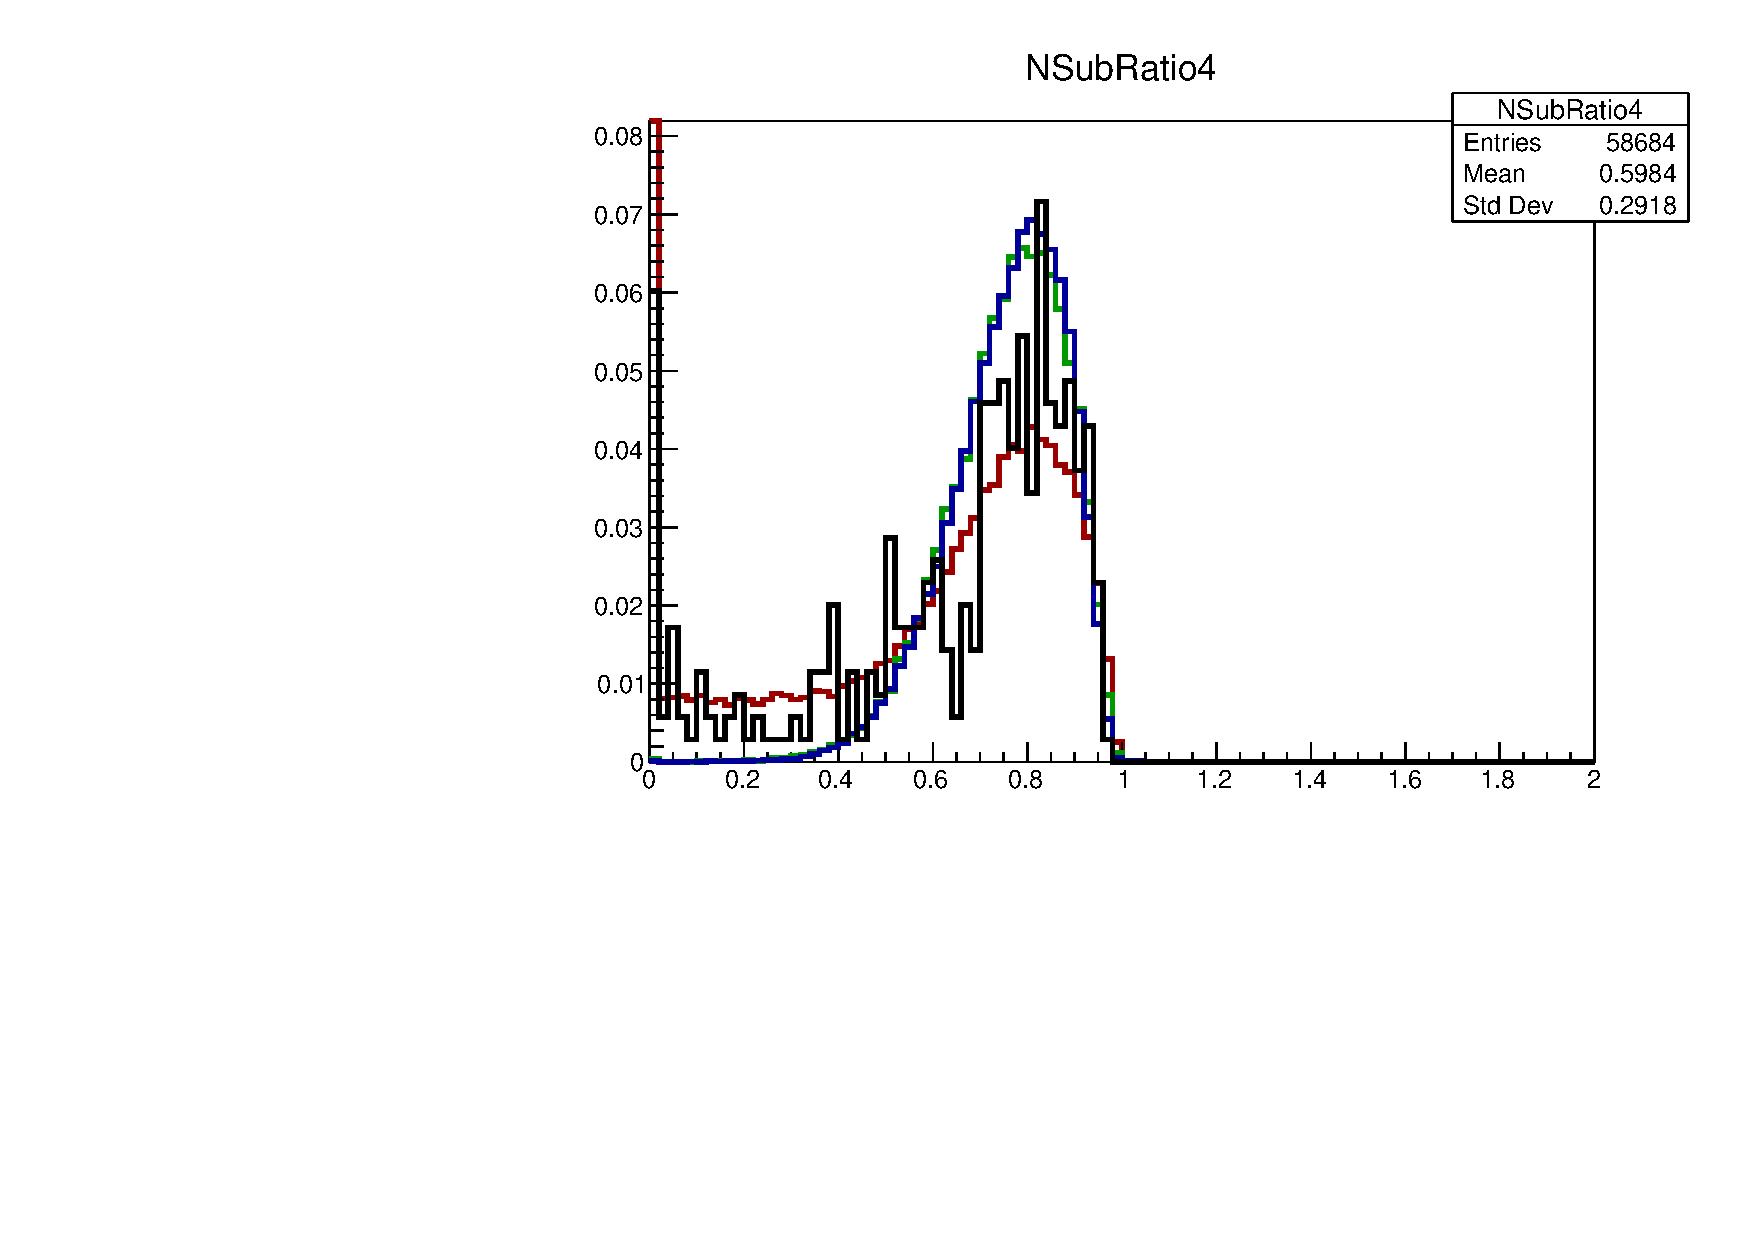
\includegraphics[width=0.49\textwidth]{./NSubRatio4.pdf}\\
        \caption{ Ratio of {\tt NSubJettiness} observable, normalized to unit area under the curve. }
        \label{fig:NSubRatio}
    \end{center}
\end{figure}
